% Source for the figure of PageHeap (sec. 5.7): a segment cut into pages of
% one class each, the current page and the list A_1 of the pages of the
% class 1 with free slots, before and after the free of a slot of the
% exhausted page P1; below, a page: its header and its slots, the slot p
% finding the page by masking its address. Build: make figures (in
% ../build).
\documentclass[border=4pt]{standalone}
\usepackage[T1]{fontenc}
\usepackage{newpxtext,newpxmath}
\usepackage[varqu,varl,scaled=0.95]{zi4}
\usepackage{tikz}
% tikz-ads.tex: the TikZ styles shared by the figures of the memory of the
% manual, \input by each standalone figure: a cell of a vector (cell), the
% cell that an operation touches (touched), a free cell (free), a node of a
% linked structure (node), the labels of indices (index) and of variables
% (var), a pointer (ptr), and \cells and \indices to draw a row of cells.
\usetikzlibrary{arrows.meta,positioning,calc,fit,shapes.multipart}
\definecolor{adsTouched}{RGB}{214,196,236}
\definecolor{adsFree}{RGB}{236,236,236}
\tikzset{
  ads/.style={>={Stealth[length=2mm]},font=\small,
              every node/.append style={inner sep=0pt}},
  cell/.style={draw,minimum width=7mm,minimum height=7mm,
               font=\small\ttfamily,outer sep=0pt},
  touched/.style={cell,fill=adsTouched},
  free/.style={cell,fill=adsFree,text=black!45},
  node/.style={draw,rounded corners=1pt,minimum width=8mm,
               minimum height=6mm,font=\small\ttfamily},
  index/.style={font=\scriptsize\ttfamily,text=black!60},
  var/.style={font=\small\itshape},
  ptr/.style={->,thick}
}
% \cells{name}{x,y}{list}: a row of cells, the first at (x,y), named
% name-0, name-1, ...; each item is text/style, the style one of cell,
% touched and free (e.g., {a/cell,e/touched,/free})
\newcommand{\cells}[3]{%
  \foreach \v/\s [count=\i from 0] in {#3}
    \node[\s] (#1-\i) at ($(#2)+(\i*7mm,0)$) {\v};}
% \indices{name}{n}: the indices 0 .. n-1 under the cells of name
\newcommand{\indices}[2]{%
  \foreach \i in {0,...,\numexpr#2-1\relax}
    \node[index,below=1.2mm of #1-\i] {\i};}

\tikzset{pg/.style={cell,minimum width=14mm,font=\scriptsize\ttfamily}}
% \seg{y}{style of P1}{text of P1}: the first pages of the segment
\newcommand{\seg}[3]{%
  \node[pg] at (0,#1) {P0 c=1};
  \node[#2,minimum width=14mm,font=\scriptsize\ttfamily] at (14mm,#1) {#3};
  \node[pg] at (28mm,#1) {P2 c=3};
  \node[pg] at (42mm,#1) {P3 c=1};
  \node[pg,fill=adsFree] at (56mm,#1) {};
  \node[font=\small] at (70mm,#1) {$\cdots$};}
\begin{document}
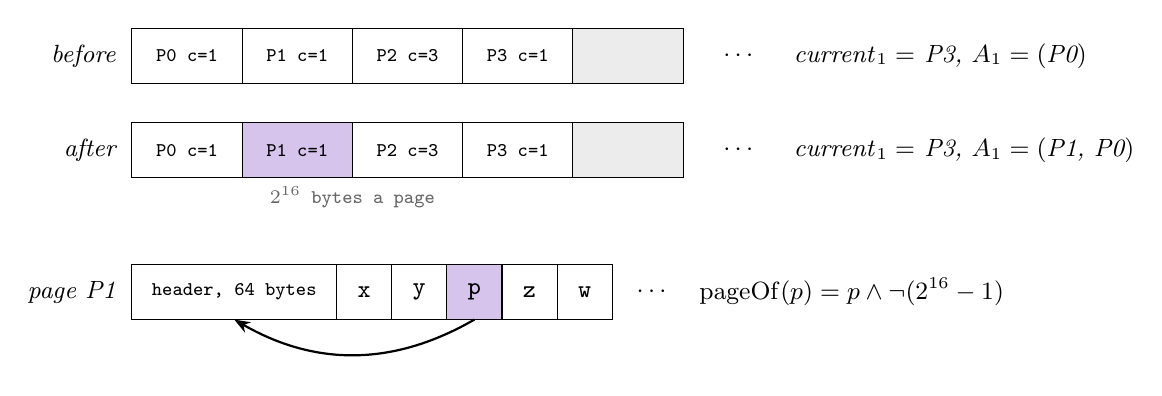
\begin{tikzpicture}[ads]
  \node[var,anchor=east] at (-9mm,0) {before};
  \seg{0}{cell}{P1 c=1}
  \node[var,anchor=west] at (77mm,0)
    {$\mathit{current}_1 = $ P3, $A_1 = ($P0$)$};
  \node[var,anchor=east] at (-9mm,-12mm) {after};
  \seg{-12mm}{touched}{P1 c=1}
  \node[var,anchor=west] at (77mm,-12mm)
    {$\mathit{current}_1 = $ P3, $A_1 = ($P1, P0$)$};
  \node[index,anchor=north] at (21mm,-16.5mm) {$2^{16}$ bytes a page};
  % a page
  \node[var,anchor=east] at (-9mm,-30mm) {page P1};
  \node[cell,minimum width=26mm,font=\scriptsize\ttfamily,anchor=west]
    (h) at (-7mm,-30mm) {header, 64 bytes};
  \cells{s}{22.5mm,-30mm}{x/cell,y/cell,p/touched,z/cell,w/cell}
  \node[font=\small] at (59mm,-30mm) {$\cdots$};
  \node[var,anchor=west] at (65mm,-30mm)
    {$\mathrm{pageOf}( p ) = p \wedge \neg ( 2^{16} - 1 )$};
  \draw[ptr] (s-2.south) to[bend left=30] (h.south);
\end{tikzpicture}
\end{document}
